\begin{figure}[H]
    \begin{subfigure}[t]{\textwidth}
        \caption{}
        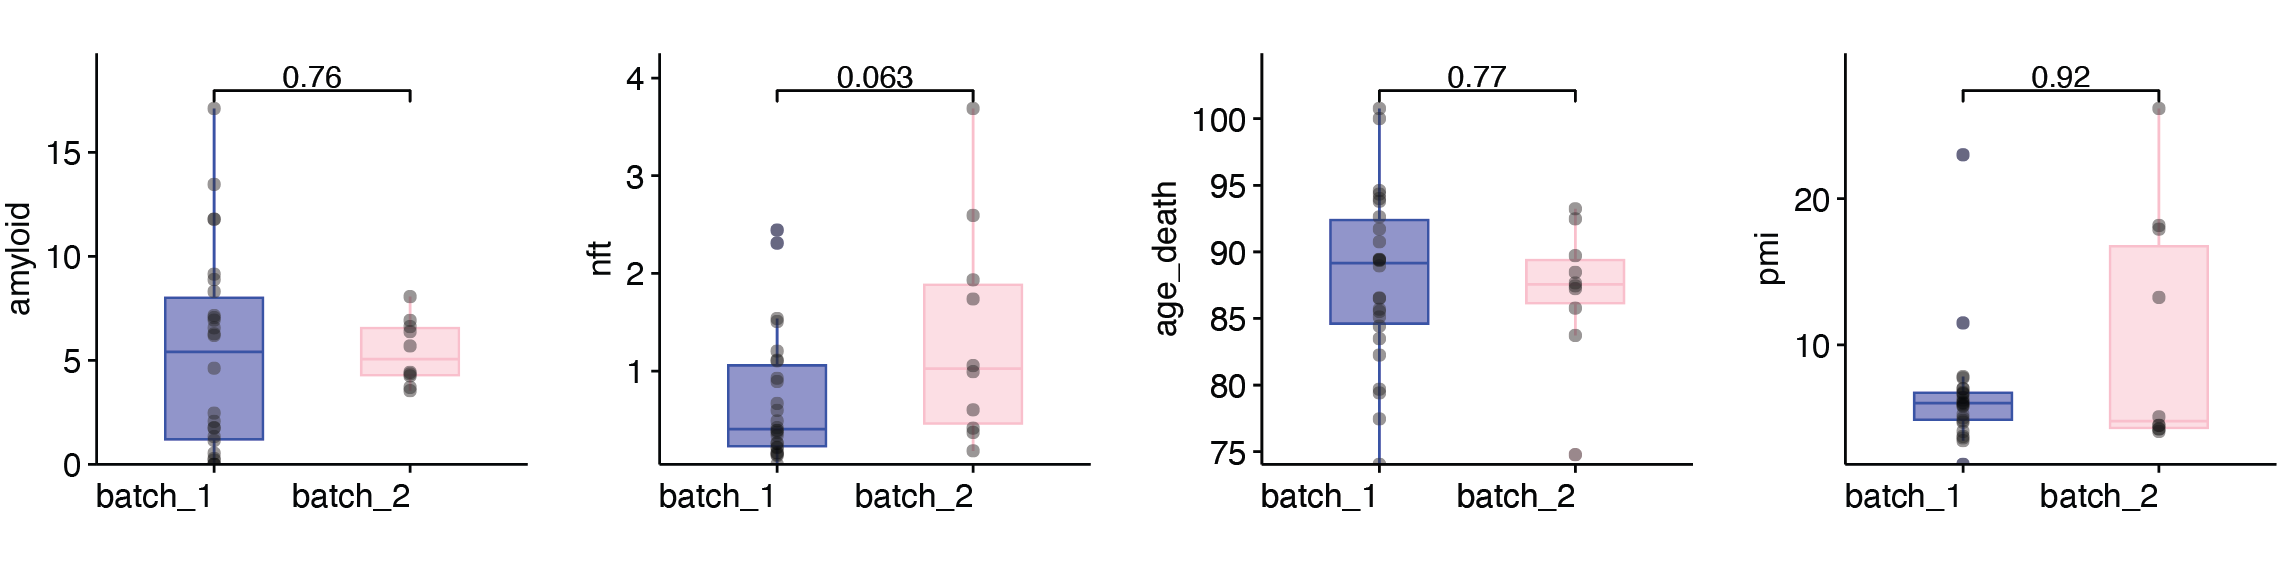
\includegraphics[width=\textwidth]{../paper/extended_plots/seq_batch_cont.png}        
    \end{subfigure}
    \begin{subfigure}[t]{\textwidth}
        \caption{}
        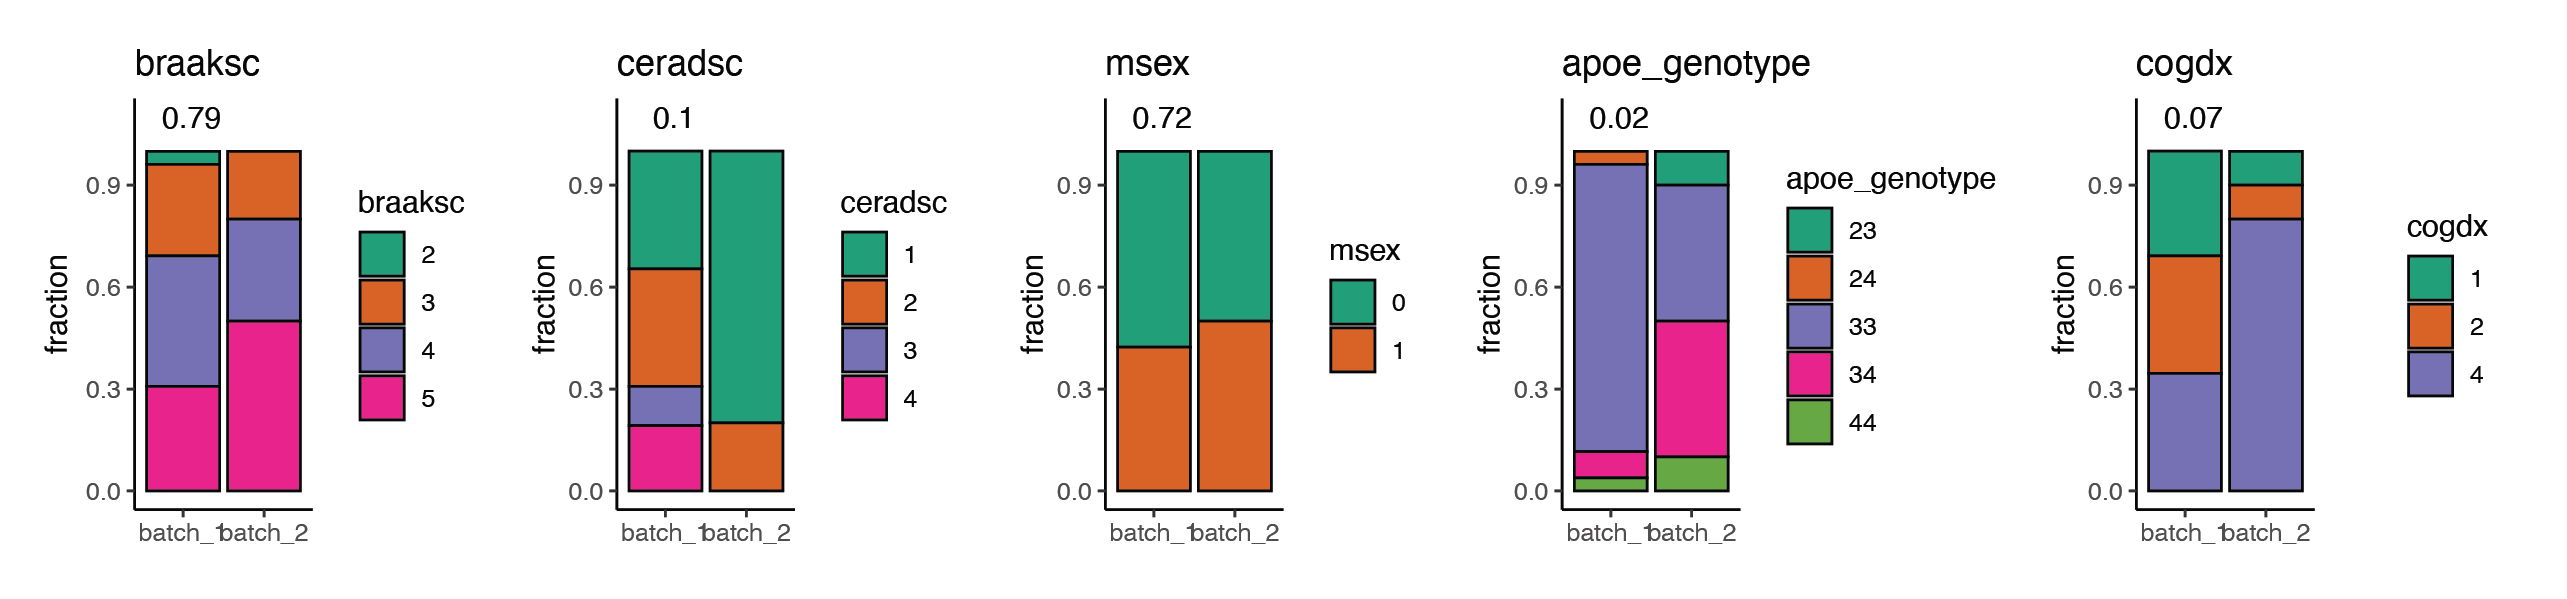
\includegraphics[width=\textwidth]{../paper/extended_plots/seq_batch_cat.png}        
    \end{subfigure}  
    \begin{subfigure}[t]{\textwidth}
        \caption{}
        \includegraphics[width=\textwidth]{../paper/extended_plots/additional_projections.png}        
    \end{subfigure}   
    \begin{subfigure}[t]{\textwidth}
        \caption{}
        \includegraphics[width=\textwidth]{../paper/extended_plots/score_correlations_by_batch.png}        
    \end{subfigure}   
\end{figure}
\textbf{Fig. S2: Overview of snRNA-sequencing Batch Correction and Data Quality.}
\textbf{a,} Distribution of continuous metadata variables by sequencing batch. P-values in panels were computed by two-sided Wilcoxon rank sum test.
\textbf{b,} Distribution of discrete metadata variables by sequencing batch. P-values were computed by two-sided Fisher's exact test.
\textbf{c,} 2D UMAP projection of snRNA-seq cells after quality control, colored by selected metadata variables.
\textbf{d,} Correlation of gene perturbation scores ($S = -\log_{10}(p)\times\text{sign}(\log_2(\text{fold-change}))$) computed using all samples versus excluding batch 2 (v2 chemistry), demonstrating that results are robust and not driven by batch-specific effects.
